\documentclass{standalone}
\usepackage{tikz}
\begin{document}

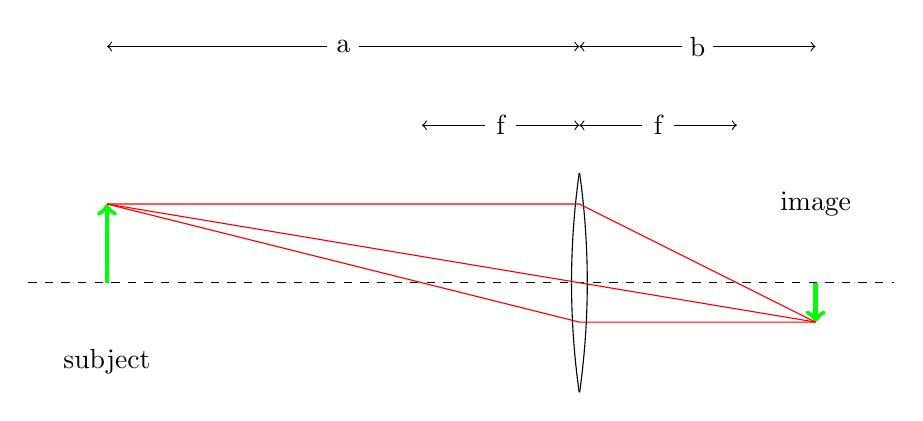
\begin{tikzpicture}

%\namedhorline{text}{textpos}{radius}
\newcommand*{\namedhorline}[3]{%
	%\draw [<-] ++ -- ++(\dx,\dy) -- ++(\dx,-\dy) -- ++(-\dx,-\dy) -- cycle
	\draw [->] (#2) +(-0.2,0) -- +(-#3,0);
	\node at (#2) {#1};
	\draw [->] (#2) +(0.2,0) -- +(#3,0);
}

\def\rad{10}
\def\ang{8}

\def\lensx{0}
\def\lensy{0}
\def\lensw{0.2}

\def\objh{1}
\def\imgh{0.5}
\def\objx{6}
\def\imgx{3}
\def\f{2}
% 1/3 + 1/6 = 1/2

\def\flabely{2}
\def\alabely{3}

% background
\draw [dashed] (-\objx-1, 0) -- (\imgx+1, 0);

% lens

\draw (\lensx+\lensw/2,\lensy) arc [radius=\rad, start angle=0, end angle=\ang];
\draw (\lensx+\lensw/2,\lensy) arc [radius=\rad, start angle=0, end angle=-\ang];

\draw (\lensx-\lensw/2,\lensy) arc [radius=\rad, start angle=180, end angle=180+\ang];
\draw (\lensx-\lensw/2,\lensy) arc [radius=\rad, start angle=180, end angle=180-\ang];
%\draw (\lensx-\lensw/2,\lensy) arc [radius=\rad, start angle=180-\ang, end angle=180+\ang];

% object, image
\draw [green, ultra thick, ->] (-\objx, 0) -- (-\objx, \objh);
\draw [green, ultra thick, ->] (\imgx, 0) -- (\imgx, -\imgh);

% light beams
\draw [red] (-\objx, \objh) -- (\lensx, \lensy+\objh) -- (\imgx, -\imgh);
\draw [red] (-\objx, \objh) -- (\imgx, -\imgh); % thru the lens center
\draw [red] (-\objx, \objh) -- (\lensx, \lensy-\imgh) -- (\imgx, -\imgh);

% labels

\namedhorline{f}{-1,\flabely}{1}
\namedhorline{f}{1,\flabely}{1}

\namedhorline{a}{-3,\alabely}{3}

\node at (-\objx, -1) {subject};
\node at (\imgx, 1) {image};

\namedhorline{b}{1.5,\alabely}{1.5}

\end{tikzpicture}

\end{document}
